\documentclass[12pt,a4paper]{article}

\usepackage[margin=1in]{geometry}
\usepackage{graphicx}
\usepackage{verbatim}
\usepackage{iftex}
\usepackage{float}
\usepackage[hidelinks]{hyperref}
\usepackage{xurl}
\urlstyle{same}
\sloppy

\ifPDFTeX
  \usepackage{helvet}
  \usepackage{courier}
  \renewcommand{\familydefault}{\sfdefault}
\else
  \usepackage{fontspec}
  \setmainfont{Arial}
  \setsansfont{Arial}
  \IfFontExistsTF{Consolas}{\setmonofont{Consolas}}{\setmonofont{Courier New}}
\fi

\makeatletter
\def\verbatim@font{\normalfont\ttfamily\fontsize{10}{12}\selectfont}
\renewcommand\section{\@startsection{section}{1}{\z@}%
  {-3.5ex \@plus -1ex \@minus -.2ex}%
  {2.3ex \@plus .2ex}%
  {\normalfont\bfseries\fontsize{14}{16}\selectfont}}
\renewcommand\subsection{\@startsection{subsection}{2}{\z@}%
  {-3.25ex \@plus -1ex \@minus -.2ex}%
  {1.5ex \@plus .2ex}%
  {\normalfont\bfseries\fontsize{12}{14}\selectfont}}
\makeatother

\title{CPT304 Coursework 1 Report\\Taskify Research-Led Software Enhancement}
\author{Group 13}
\date{May 2026}

\begin{document}
\maketitle

\section{App Selection}
We chose Taskify because it already behaved like a real web application, but it
still had obvious weaknesses once we started testing it properly. The project
had an Express backend, authentication pages, a dashboard, automated tests, and
a live Vercel deployment, so we could inspect the code, reproduce the problems
in the browser, and keep evidence for each change. In the first audit, we
identified four specific deficiencies:
placeholder-only form fields, missing backend form handlers, dashboard state
loss after refresh, and weak task feedback. That made the project suitable for
this coursework because the issues were real enough to analyse, but still small
enough to fix and verify within the report.

\noindent\textbf{Direct GitHub PR links for verification.} Auth form
accessibility: \url{https://github.com/maoyouaa/Taskify/pull/1}; dashboard
persistence: \url{https://github.com/maoyouaa/Taskify/pull/3}; task
feedback/actions: \url{https://github.com/maoyouaa/Taskify/pull/4}; auth form
POST routes: \url{https://github.com/maoyouaa/Taskify/pull/5}; bilingual
language toggle evidence: \url{https://github.com/maoyouaa/Taskify/pull/6}.

\section{Authentication Form Fields Relied on Placeholder Text}

\subsection{Detection}
The first problem was detected with browser DevTools inspection of the rendered
sign-up form and its markup. Each account field
used placeholder text as the only visible label. That meant the field name
disappeared as soon as the user started typing, which is awkward even in a
simple form. We typed into the username field, observed the placeholder vanish
in the browser, and then checked all five account inputs to confirm that the
same issue affected \texttt{SignUpUsername}, \texttt{SignUpEmail},
\texttt{SignUpPassword}, \texttt{LoginEmail}, and \texttt{LoginPassword}.
Figure~\ref{fig:auth-form-labels} records that before-and-after state for
verification.

\subsection{Literature}
The accessibility sources we used all pointed in the same direction. W3C WAI's
forms tutorial recommends a visible label that is tied to the input with
matching \texttt{for} and \texttt{id} attributes \cite{w3c-labels}. WebAIM
makes the practical point that placeholders are useful as hints, but they are
not a substitute for labels because they disappear while the form is being
filled in \cite{webaim-forms}. W3C's explanation of WCAG 2.2 Success Criterion
3.3.2 says the same thing in a more formal way: labels should remain available
as instructions, not vanish with the placeholder \cite{w3c-sc332}. That was the
basis for the fix.

\subsection{Implementation}
The original email field depended on the placeholder for its meaning:

\noindent\textbf{Before fix: placeholder-only email field.}
{\footnotesize
\begin{verbatim}
<input type="email" name="SignUpEmail"
  placeholder="Email" required="true" />
\end{verbatim}
}

We changed the form so the label stays visible and the hint becomes secondary:

\noindent\textbf{After fix: visible label connected to the input.}
{\footnotesize
\begin{verbatim}
<label class="field-label" for="signup-email">Email</label>
<input id="signup-email" type="email" name="SignUpEmail"
  autocomplete="email" placeholder="Email" required />
\end{verbatim}
}

The same pattern was applied to the other account fields in the sign-up
template. We also split the CSS so \texttt{.toggle-label}
still styles the Sign Up / Log In switch, while \texttt{.field-label} styles
the ordinary form labels. After that change, the form kept a stable label after
typing, and the accessibility tree exposed clearer names such as
\texttt{textbox "User name"} and \texttt{textbox "Email"}.

\begin{figure}[H]
  \centering
  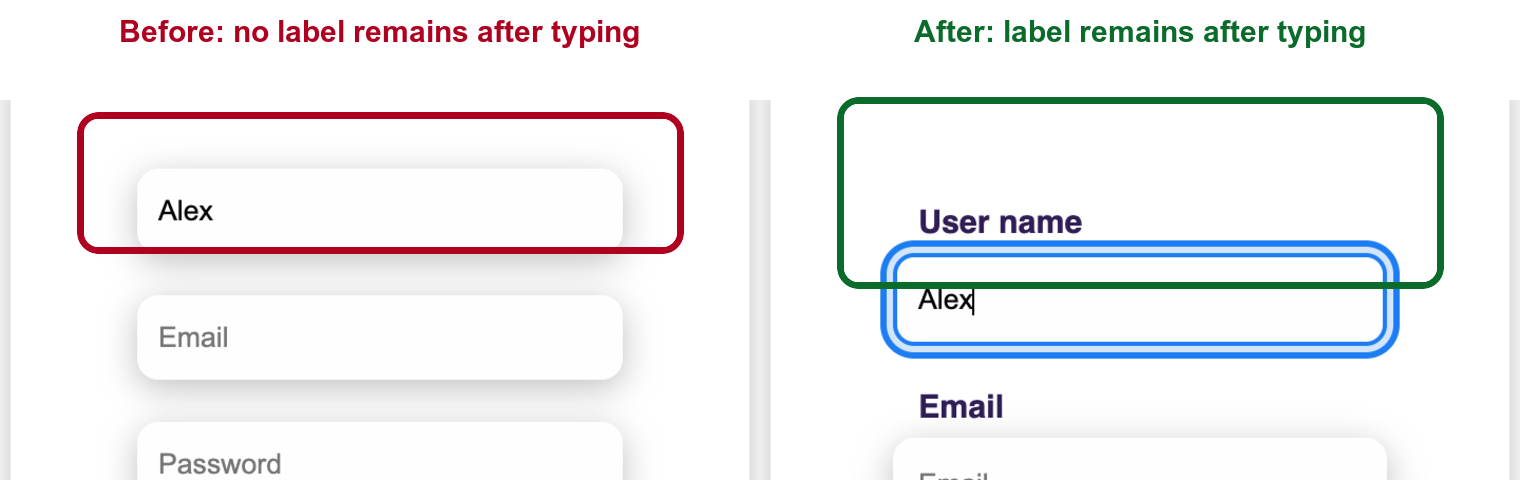
\includegraphics[width=0.92\linewidth]{figures/auth-form-labels-before-after.png}
  \caption{Authentication form label evidence. Before the fix, the username placeholder disappears after typing and no field label remains. After the fix, the visible ``User name'' label stays above the filled input.}
  \label{fig:auth-form-labels}
\end{figure}

\section{Authentication Forms Submitted to Missing Backend Routes}

\subsection{Detection}
The second deficiency appeared when we compared the frontend forms with the
server routes. The page submitted \texttt{POST /signup} and
\texttt{POST /login}, but the earlier server setup only defined GET routes for
the page views. That meant the interface looked complete even though the
backend could not process either form. We confirmed this by sending a signup
request and receiving \texttt{HTTP/1.1 404 Not Found}, as shown in
Figure~\ref{fig:auth-http-evidence}.

\subsection{Literature}
The implementation decision here came from a mix of framework documentation and
security guidance. Express explains that routes are matched by both path and
HTTP method, so \texttt{GET /signup} cannot handle a \texttt{POST /signup}
submission \cite{express-routing}. OWASP's Input Validation Cheat Sheet also
states that browser-side checks are not enough on their own, because the server
still needs to validate untrusted input \cite{owasp-input-validation}. Finally,
MDN's explanation of \texttt{303 See Other} gave us a clean way to return the
user to a GET page after a successful POST request \cite{mdn-303}.

\subsection{Implementation}
Originally, the sign-up page could render, but it could not accept its own form
submission:

\noindent\textbf{Before fix: sign-up page existed, but no POST handler existed.}
{\footnotesize
\begin{verbatim}
app.get("/signup", (req, res) => {
    res.status(200).render("signup.ejs");
});
\end{verbatim}
}

We added explicit POST handlers with server-side validation and redirect logic:

\noindent\textbf{After fix: server-side validation and Post/Redirect/Get.}
{\footnotesize
\begin{verbatim}
app.post("/signup", (req, res) => {
    const missingFields = collectMissingFields(req.body, [
        "SignUpUsername", "SignUpEmail", "SignUpPassword",
    ]);

    if (missingFields.length > 0 || !isValidEmail(req.body.SignUpEmail)) {
        return res.status(400).json({
            success: false,
            errors: {
                missingFields,
                email: isValidEmail(req.body.SignUpEmail) ? undefined
                    : "Enter a valid email address.",
            },
        });
    }

    return res.redirect(303, "/dashboard");
});
\end{verbatim}
}

The same approach was added for \texttt{POST /login}. After the change, a valid
signup request returned \texttt{303 See Other} with
\texttt{Location: /dashboard}, while an invalid email produced
\texttt{400 Bad Request} and an error message. The later hardening work then
extended this flow by storing registered-user passwords as hashes and requiring
a signed session cookie before \texttt{/dashboard} could be opened
\cite{owasp-authentication,owasp-session-management}. We also exported the app
and only called \texttt{listen()} when run directly, so the route tests could
run against a temporary server.

\begin{figure}[H]
  \centering
  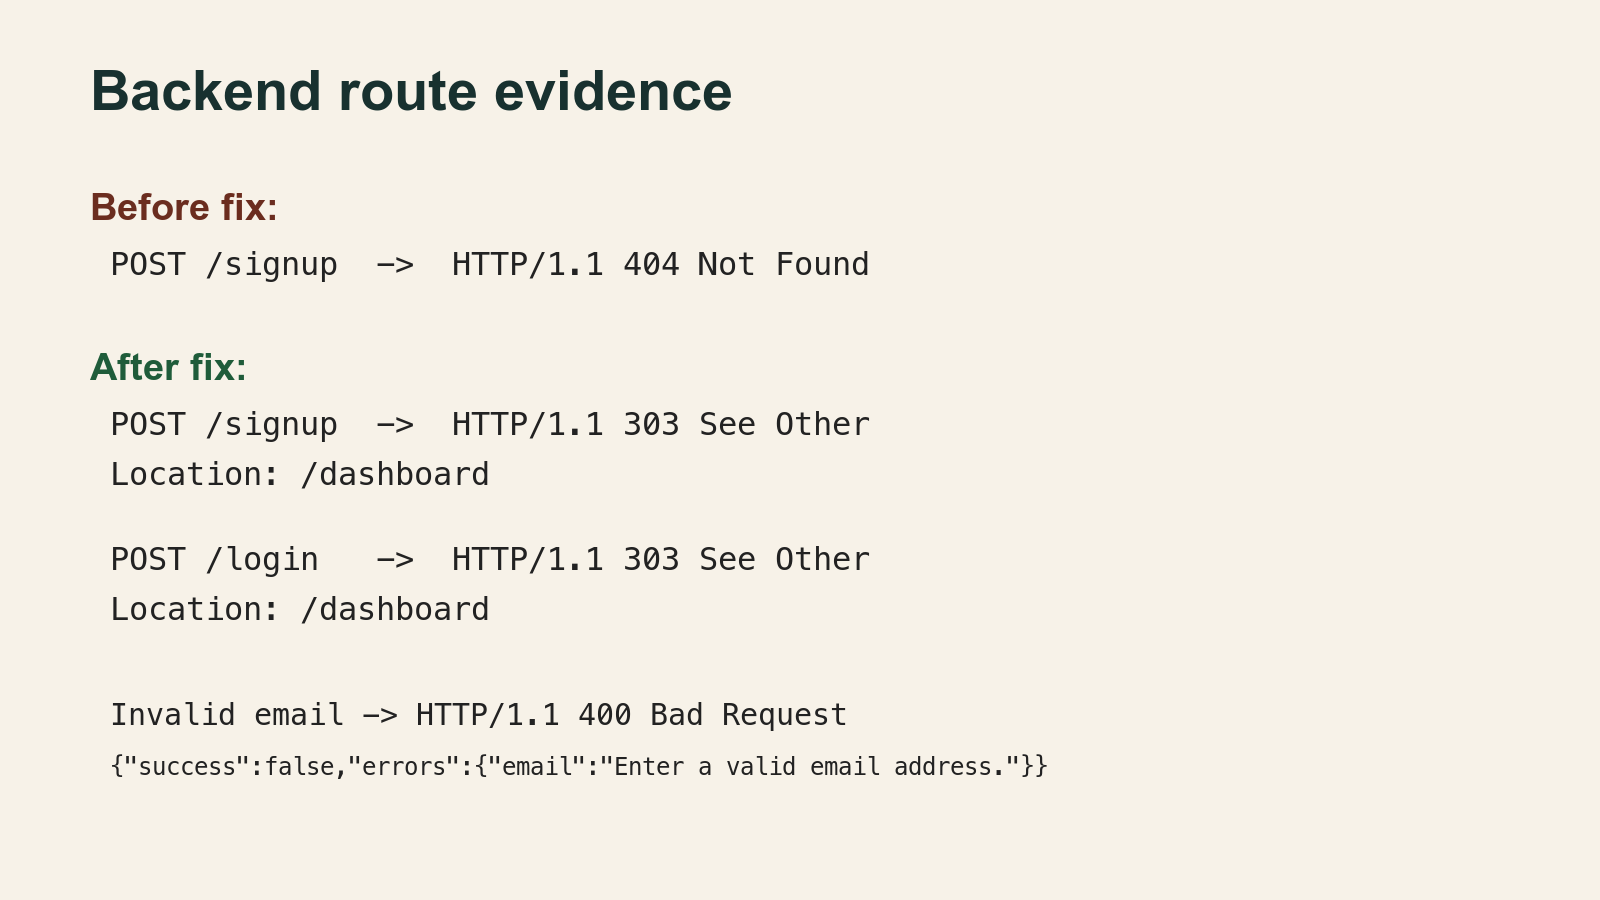
\includegraphics[width=0.92\linewidth]{figures/auth-http-evidence.png}
  \caption{Backend route evidence. Before the fix, \texttt{POST /signup} returned 404. After the fix, valid submissions redirect to \texttt{/dashboard} with \texttt{303}, while invalid email input returns \texttt{400}.}
  \label{fig:auth-http-evidence}
\end{figure}

\section{Dashboard Tasks Were Lost After Refresh}

\subsection{Detection}
This deficiency was detected through a browser refresh test and
\texttt{localStorage} inspection. We added and edited tasks on
\texttt{/dashboard}, refreshed the page, and compared the rendered board with
the stored task payload. The board returned to the seeded example data, which
meant the interface gave the impression that tasks had been saved even though
the state only existed in memory. When we then checked the dashboard script,
the reason was obvious: \texttt{state.tasks}
was rebuilt from \texttt{seedTasks} on every page load and nothing wrote the
latest task array to persistent storage.

\subsection{Literature}
The research for this fix was quite straightforward. MDN explains that
\texttt{localStorage} keeps browser data for the same origin across refreshes
and later sessions, so it is suitable for lightweight client-side persistence
\cite{mdn-localstorage}. web.dev adds an important warning: stored data should
not be trusted blindly, and the application should recover safely when the
stored value is missing or malformed \cite{webdev-storage}. We took those two
points as the design rule for this deficiency: save the task array after each
change, but validate any stored data before using it.

\subsection{Implementation}
In the earlier version, the dashboard always started from the same built-in task
list:

\noindent\textbf{Before fix: dashboard state was recreated on every load.}
{\footnotesize
\begin{verbatim}
let state = {
  tasks: seedTasks.map((task) => ({ ...task })),
};

function deleteTask(taskId) {
  state.tasks = state.tasks.filter((task) => task.id !== taskId);
  renderBoard();
  showMessage("Task deleted successfully.");
}
\end{verbatim}
}

We moved persistence into a small module and restored saved tasks when valid
browser storage was available:

\noindent\textbf{After fix: state is loaded safely and saved after changes.}
{\footnotesize
\begin{verbatim}
import { persistTasks, safeLoadTasks } from "./modules/task-store.mjs";

let state = {
  tasks: safeLoadTasks(window.localStorage,
    seedTasks.map((task) => ({ ...task }))).tasks,
};

function persistState() {
  persistTasks(window.localStorage, state.tasks);
}

function deleteTask(taskId) {
  state.tasks = state.tasks.filter((task) => task.id !== taskId);
  persistState();
  renderBoard();
}
\end{verbatim}
}

The storage key is \texttt{taskify.dashboard.tasks}. The verification trace
gave a concrete result rather than a vague claim: \texttt{Injected task count:
1}, \texttt{Task cards after reload: 1}, and the same JSON payload still
present after refresh. The restored task also kept the title
\texttt{Persist after refresh}, status
\texttt{doing}, priority \texttt{high}, owner \texttt{Member D}, and due date
\texttt{2026-05-11}. That matters because it shows that both the rendered board
and the stored data survived the reload. In code, \texttt{safeLoadTasks()}
wraps \texttt{JSON.parse} in a guarded fallback path, while
\texttt{persistState()} runs after save, delete, and move actions. We also
switched the dashboard script to \texttt{type="module"}, and dedicated module
tests cover the missing-storage and malformed-JSON cases.

\begin{figure}[H]
  \centering
  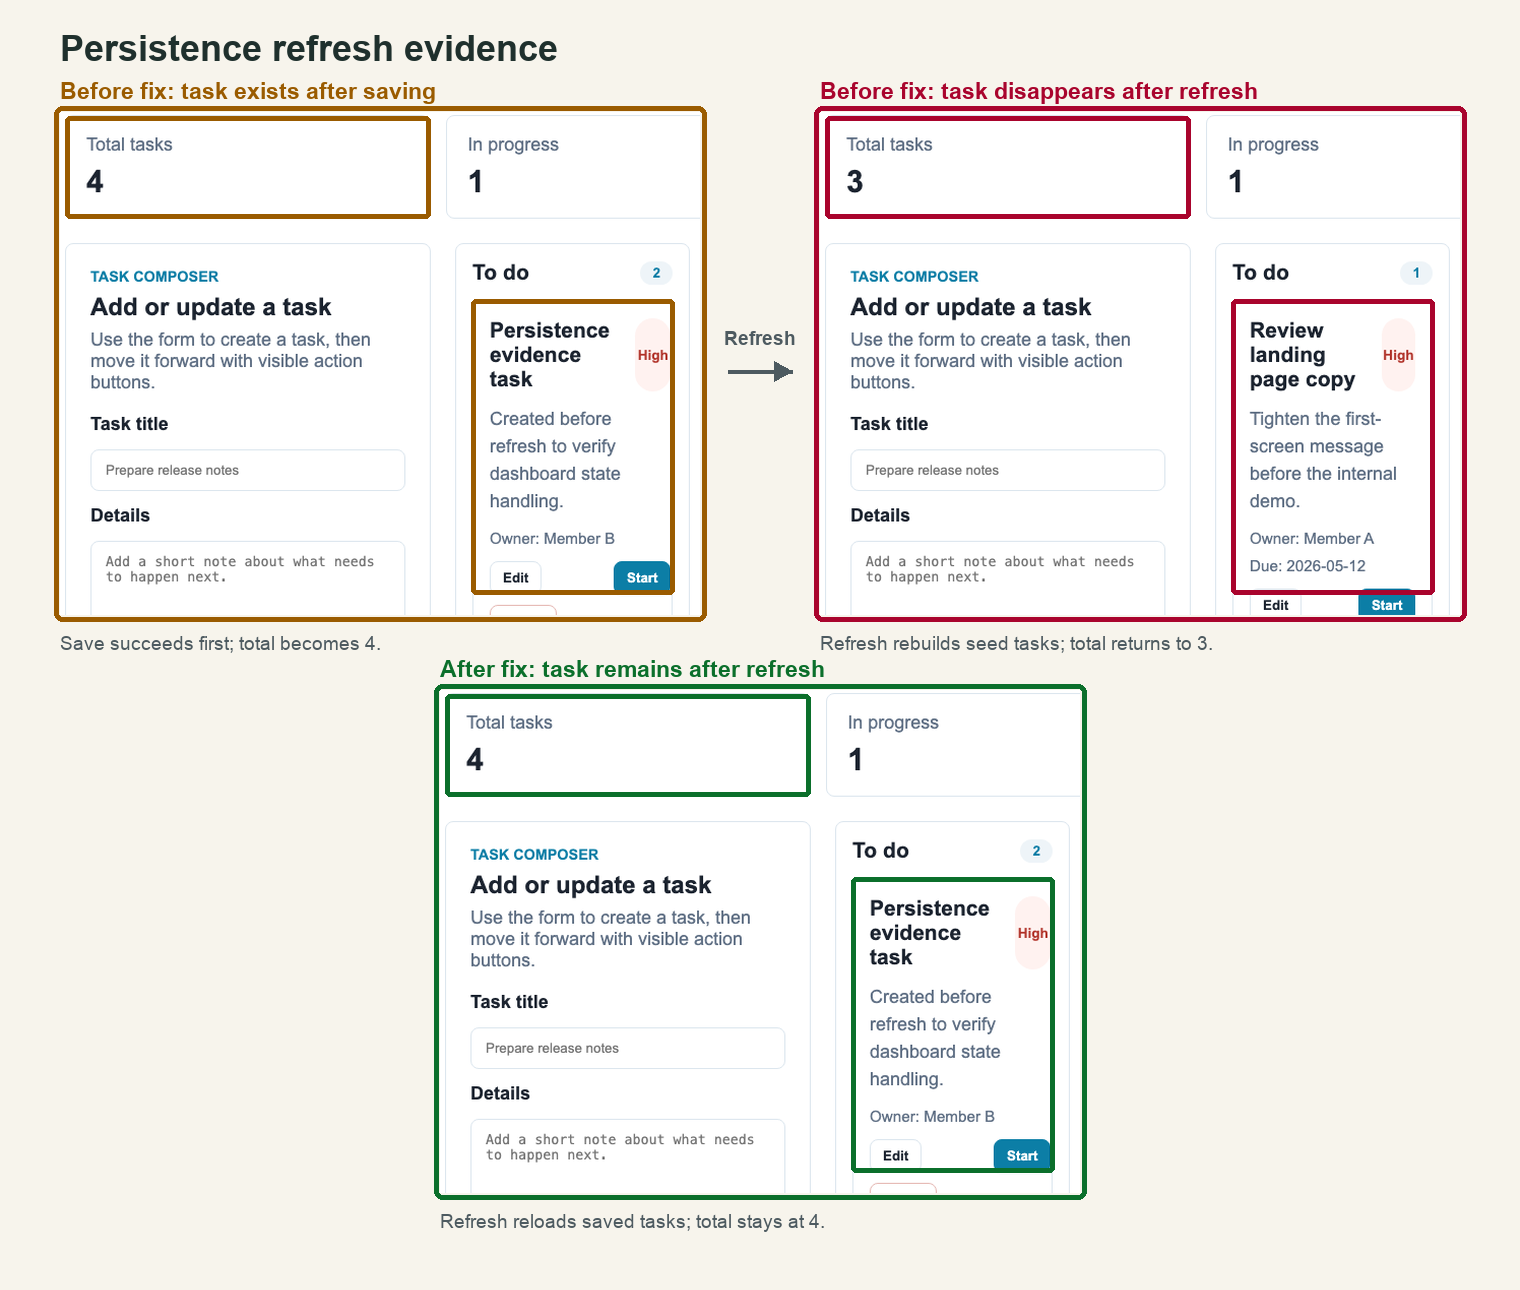
\includegraphics[width=0.96\linewidth]{figures/persistence-refresh-before-after.png}
  \caption{Persistence refresh evidence. Before the fix, refresh rebuilt the board from seed tasks and removed the saved task. After the fix, the same refresh reloads the \texttt{localStorage} task list and keeps the task visible.}
  \label{fig:persistence-refresh}
\end{figure}

\section{Weak User Feedback and Unclear Task Actions}

\subsection{Detection}
This issue was identified through browser interaction testing, returned-HTML
inspection, and source review of the earlier dashboard templates and scripts. In
the browser, the old task cards looked presentable but offered very little
direct control. The earlier interface had no dedicated live feedback area, and
actions such as edit, move, reset, or delete were not exposed as obvious
per-card controls. As a result, users had to guess whether something had
happened by watching for small layout changes. In a task manager, that is a
poor interaction pattern because routine actions should be explicit and easy to
confirm.

\subsection{Literature}
The research here focused on general usability principles rather than one narrow
technical bug. Barrington argues that usable systems should communicate system
state clearly and provide actions that users can understand and recover from
\cite{barrington-usable-products}. Nielsen Norman Group describes similar ideas
through the heuristics of visibility of system status and user control and
freedom \cite{nngroup-heuristics}. Taken together, these sources suggest that a
task board should not just display information. It should also show what the
user can do next and confirm the result immediately.

\subsection{Implementation}
Before the change, the dashboard was closer to a static task layout than a fully
interactive workspace:

\noindent\textbf{Before improvement: static dashboard content with limited user action flow.}
{\footnotesize
\begin{verbatim}
<div class="dashboard-task task-1">
  <div class="dashboard-task-head">
    Lorem ipsum dolor sit amet.
  </div>
  <div class="dashboard-task-description">
    Lorem ipsum dolor sit amet consectetur adipisicing elit.
  </div>
</div>
\end{verbatim}
}

We changed the task cards so they expose clear actions and the page responds to
each important change with visible feedback:

\noindent\textbf{After improvement: explicit task actions and visible feedback.}
{\footnotesize
\begin{verbatim}
actions.append(
  createActionButton("Edit", () => {
    fillForm(task);
    form.elements.title.focus();
    showMessage("Task loaded for editing.");
  })
);

if (task.status === "todo") {
  actions.append(createActionButton(
    "Start",
    () => moveTask(task.id, "doing", "Task moved to In progress."),
    "primary"
  ));
}
\end{verbatim}
}

Most of this work was done in the client-side dashboard logic, supported by
related template and CSS updates. An authenticated verification trace makes the
result measurable: after an authenticated signup flow, the signup response is
\texttt{303}, the redirected dashboard response is \texttt{200}, and the
returned HTML contains \texttt{id="form-message"},
\texttt{id="metric-total"}, \texttt{id="task-form"}, \texttt{id="board-grid"},
\texttt{dashboard-button-primary}, and
\texttt{dashboard-button-secondary}. The resulting dashboard, shown in
Figure~\ref{fig:dashboard-feedback-before-after}, renders visible controls such
as \texttt{Edit}, \texttt{Start}, \texttt{Complete}, \texttt{Reset}, and
\texttt{Delete}. This brought the interface closer to what the literature
recommends: actions are explicit, feedback is immediate, and the user is not
left guessing whether the board accepted the change. The figure captures a
concrete example: clicking \texttt{Start} moves the task to
\textit{In progress}, updates the counters, and replaces the default message
with a confirmation message.

\begin{figure}[H]
  \centering
  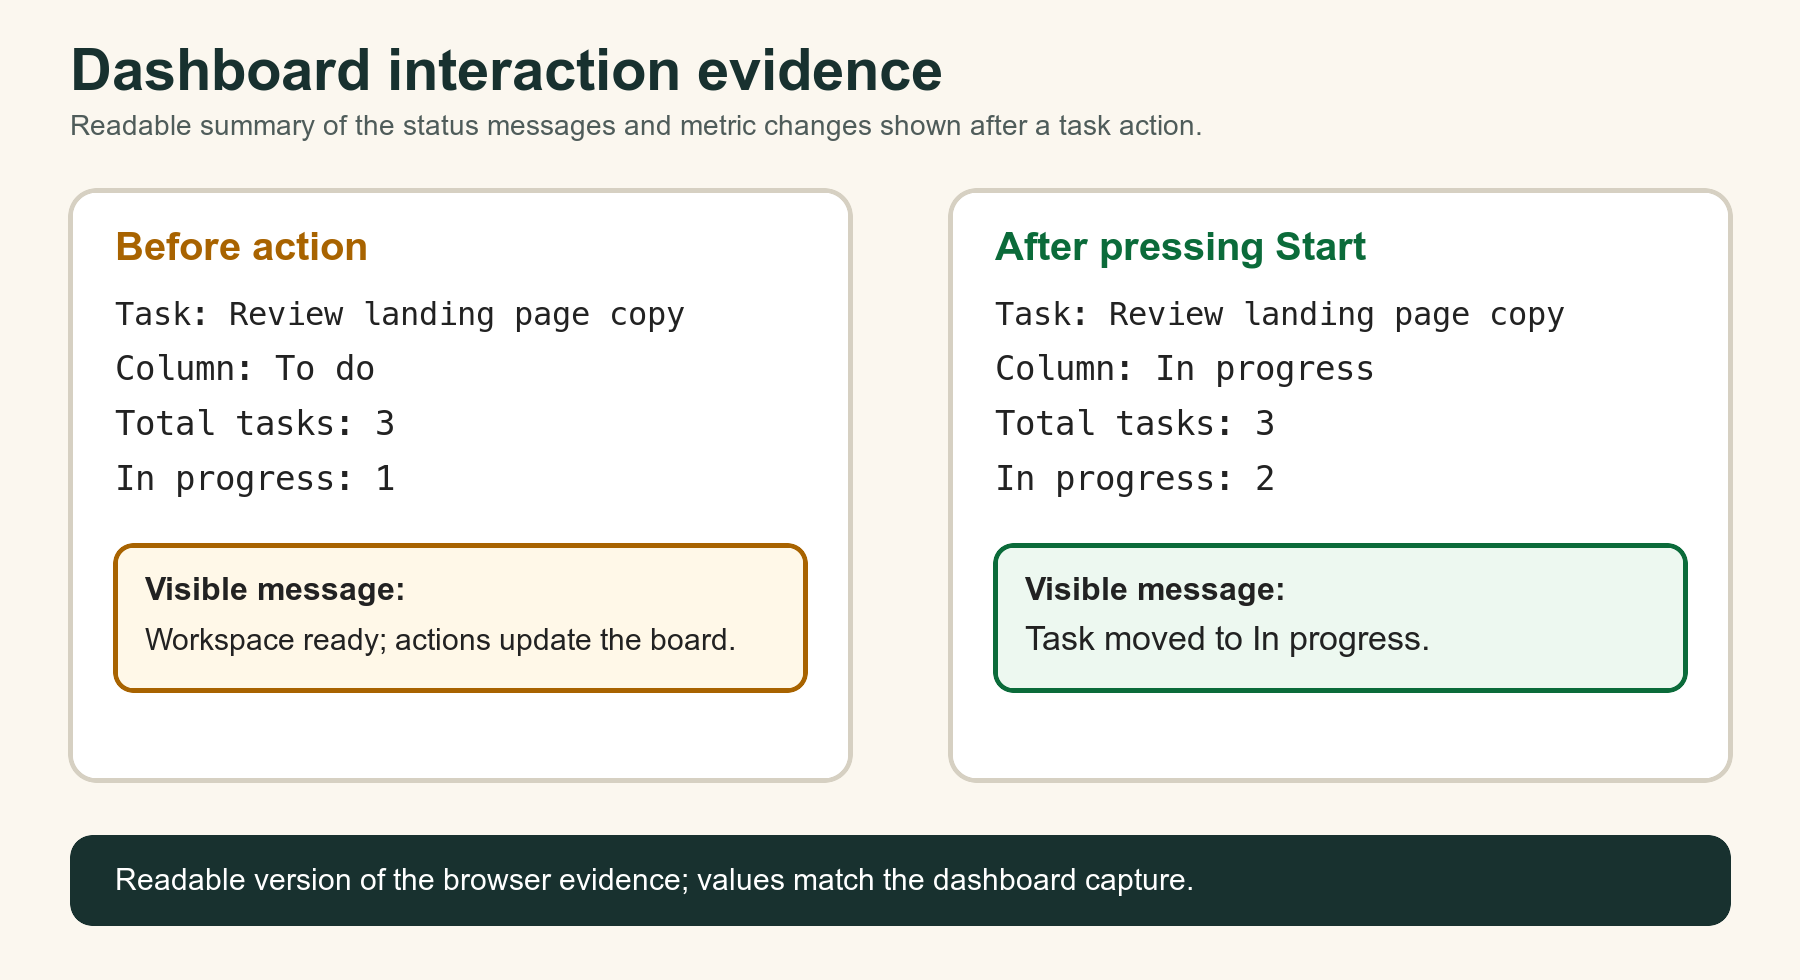
\includegraphics[width=\linewidth]{figures/dashboard-feedback-before-after.png}
  \caption{Dashboard interaction evidence. Before the fix, the task remained in the To do column and the interface showed only the default message. After \texttt{Start}, the task moves to In progress, a confirmation message appears, and the metrics update.}
  \label{fig:dashboard-feedback-before-after}
\end{figure}

\section{Baseline Standards Evidence}
The baseline standards were documented separately from the four deficiencies, as
required by the brief. Figure~\ref{fig:uptime-evidence} shows the Vercel
production history captured on 2026-05-17, including deployments aged
\texttt{7d} and \texttt{17d} and a same-day uptime confirmation from the live
site. Figure~\ref{fig:coverage-badge} shows repository coverage evidence above the required
\texttt{80\%} threshold. Figure~\ref{fig:lighthouse-score} records a Lighthouse
Accessibility score of \texttt{100}. Figure~\ref{fig:language-toggle} shows
the Chinese homepage reached through the working language toggle.
Figures~\ref{fig:cookie-banner} and \ref{fig:privacy-page} confirm the legal
baseline through a visible cookie banner and a dedicated privacy-policy page.

\begin{figure}[H]
  \centering
  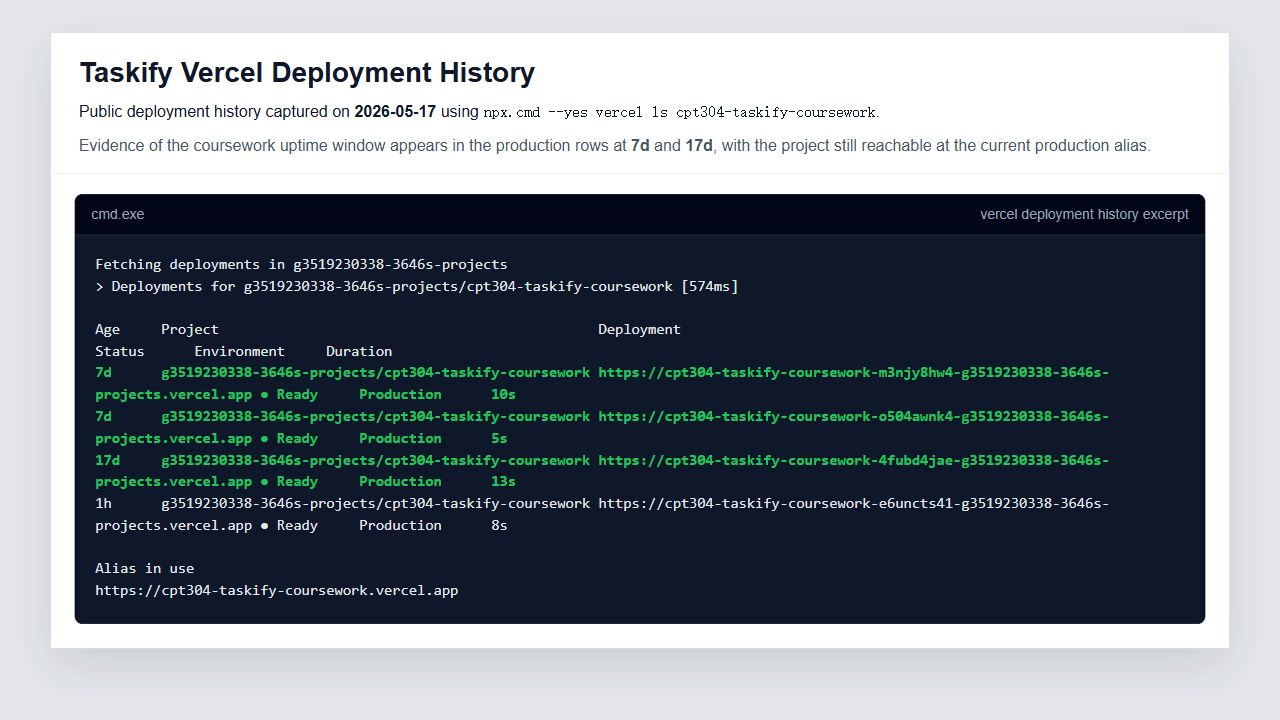
\includegraphics[width=\linewidth]{docs/baseline/evidence/vercel-7day-log.png}
  \caption{Vercel deployment-history evidence captured on 2026-05-17. The production log shows deployment ages of 7d and 17d, and the separate uptime check for the same date returned 200 OK from the production alias.}
  \label{fig:uptime-evidence}
\end{figure}

\begin{figure}[H]
  \centering
  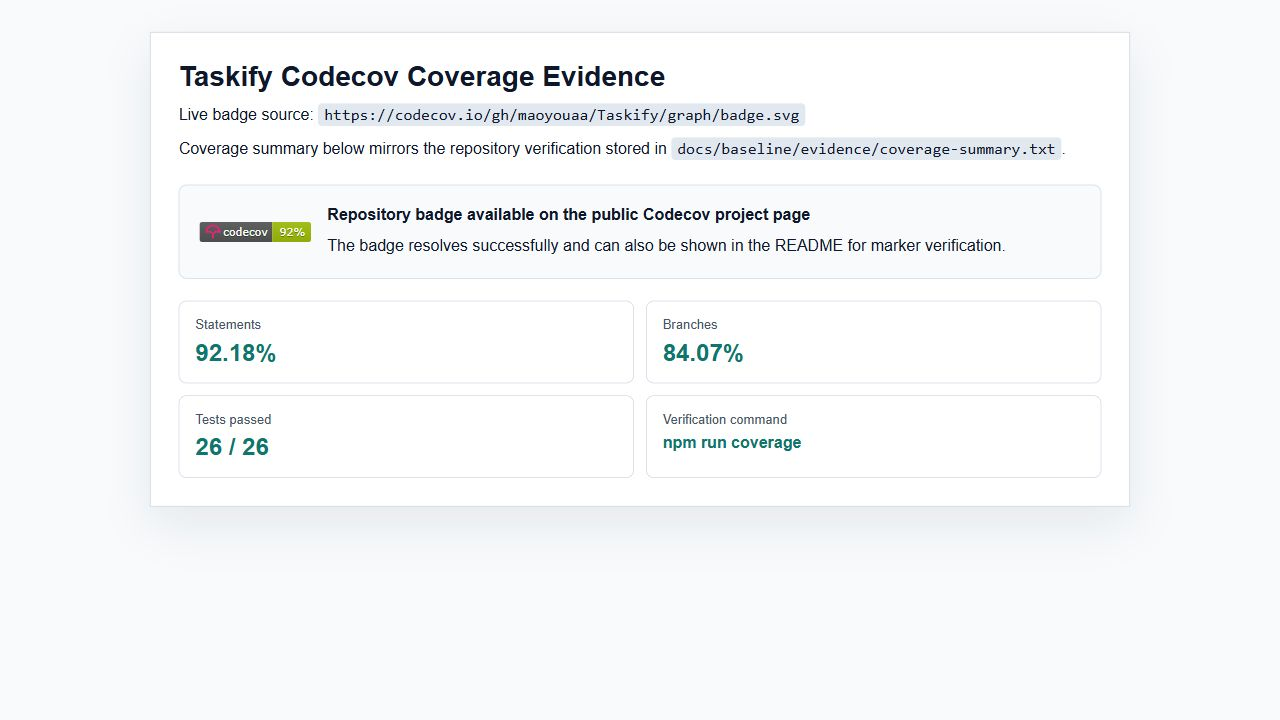
\includegraphics[width=0.72\linewidth]{docs/baseline/evidence/codecov-badge.png}
  \caption{Test-coverage evidence. This repository evidence image combines the delivered project's live Codecov badge with the current coverage-summary figures, showing coverage above the required 80\% threshold.}
  \label{fig:coverage-badge}
\end{figure}

\begin{figure}[H]
  \centering
  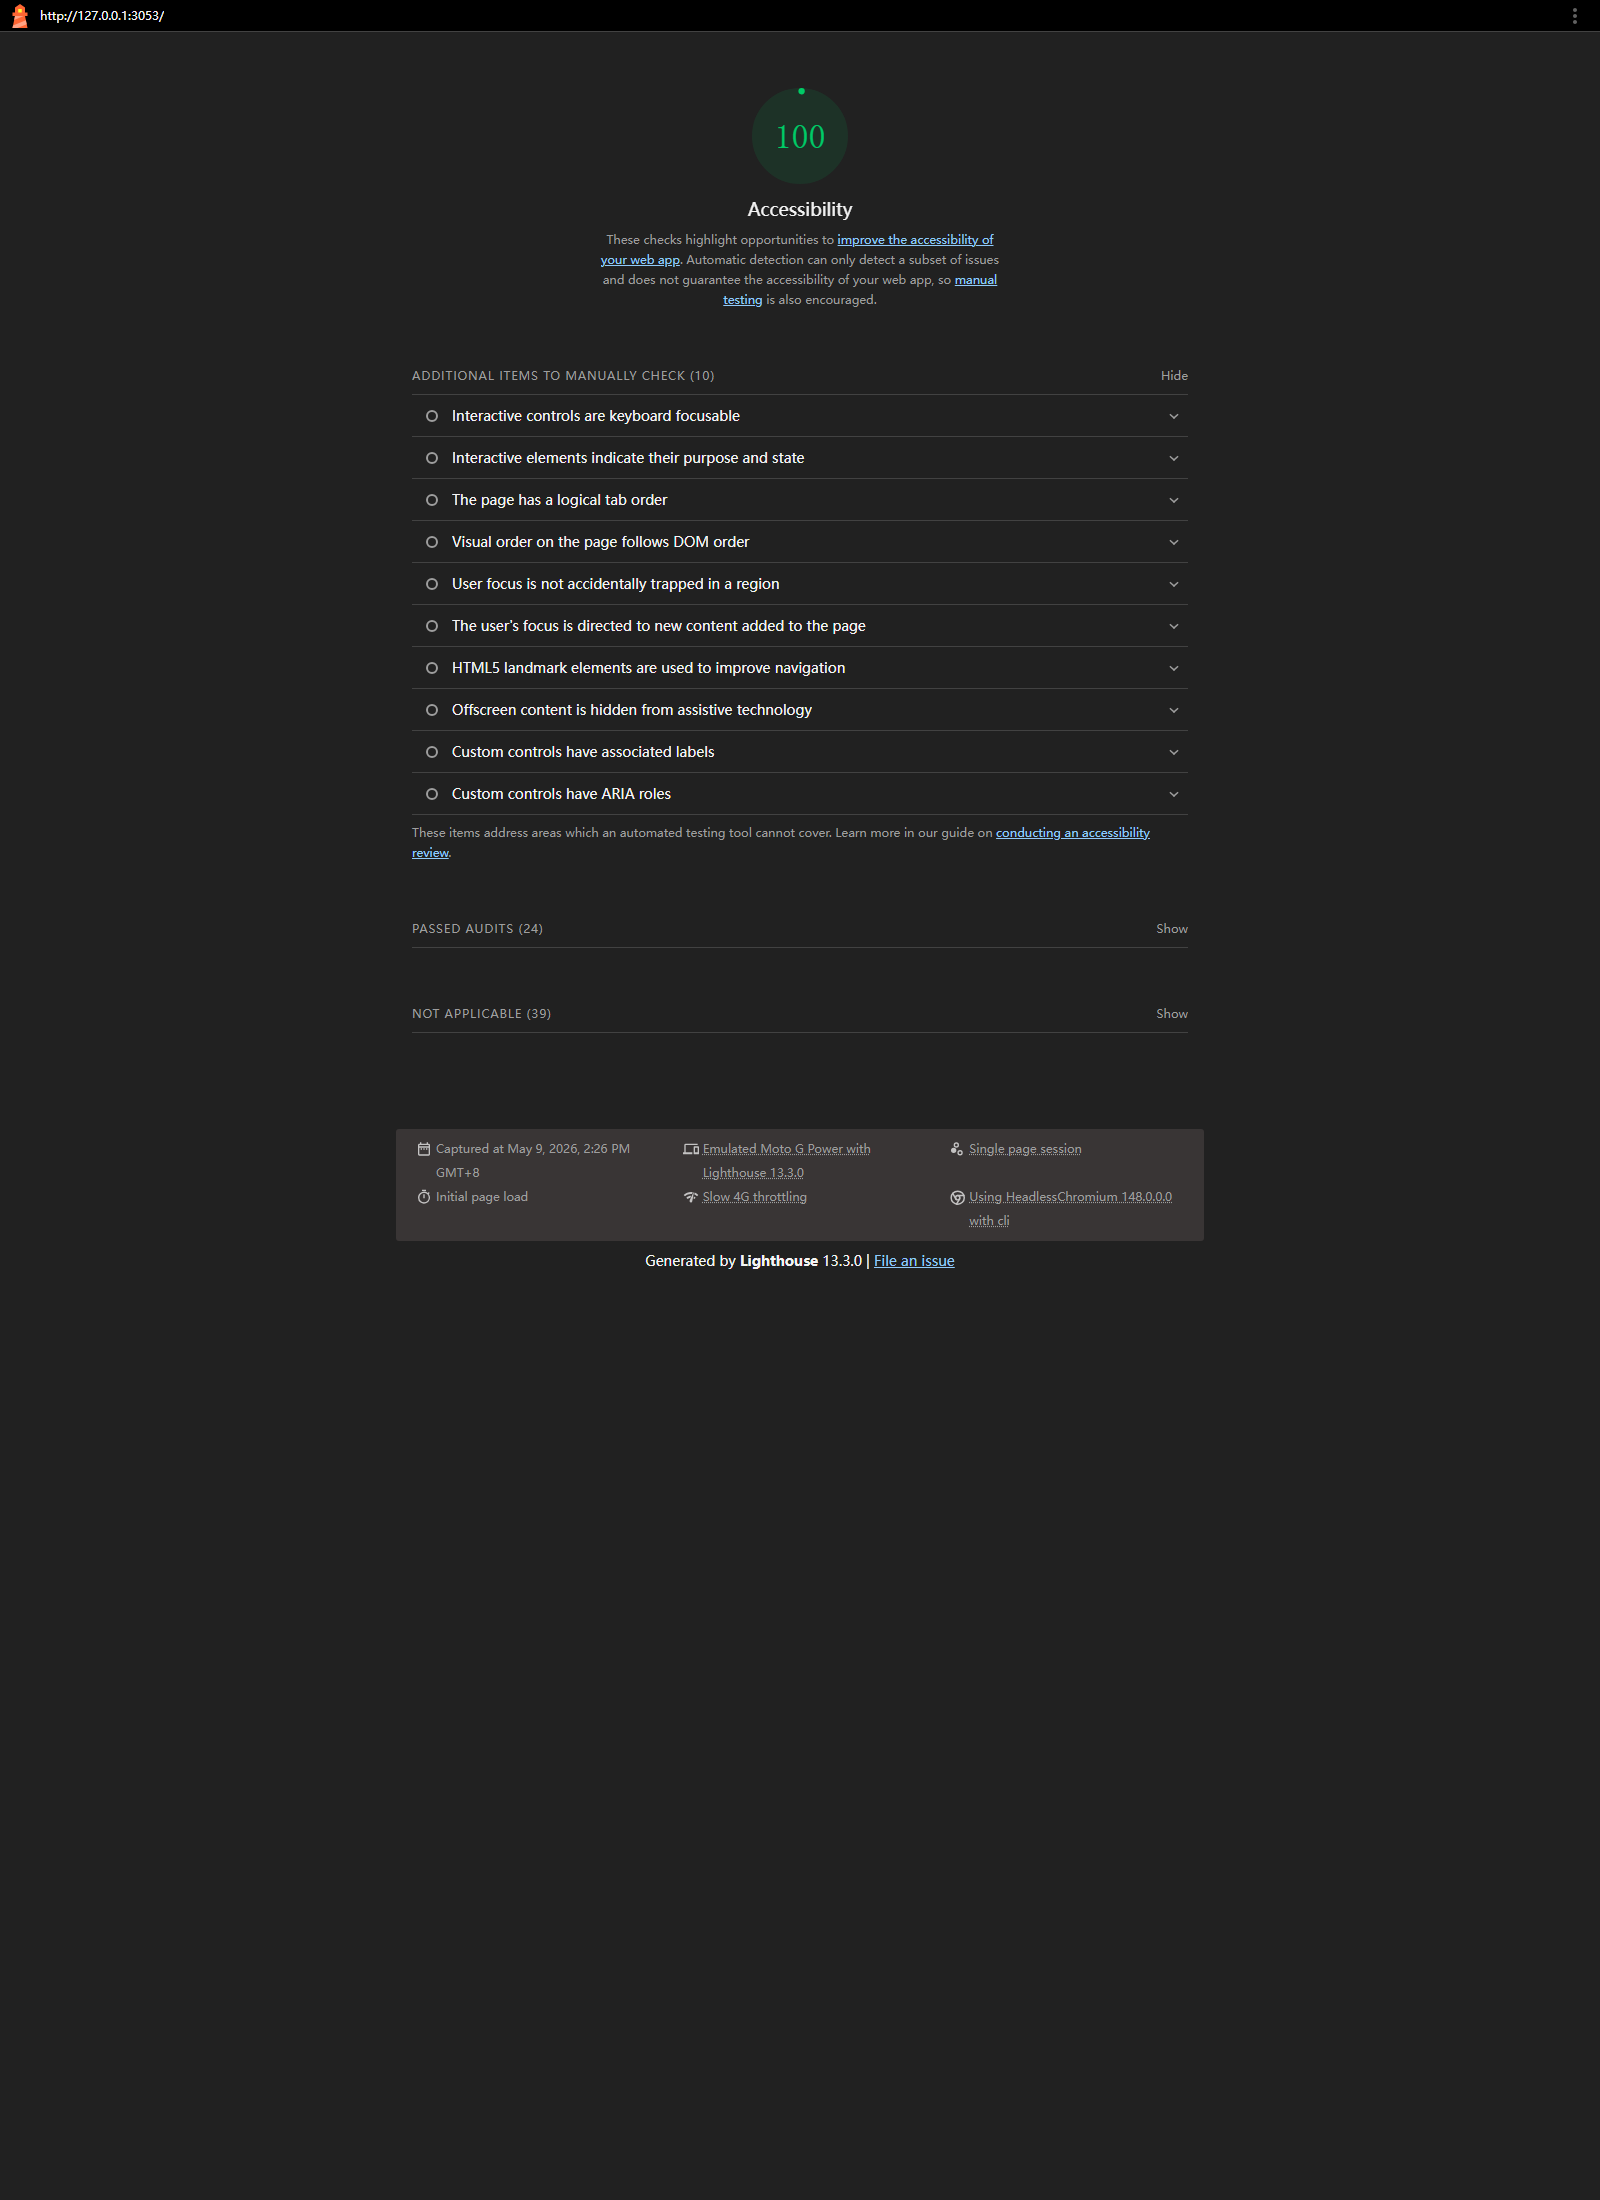
\includegraphics[width=0.92\linewidth]{docs/baseline/evidence/lighthouse-accessibility-score.png}
  \caption{Accessibility evidence. Lighthouse reports an Accessibility score of 100 for the delivered interface, which exceeds the required 90+ baseline.}
  \label{fig:lighthouse-score}
\end{figure}

\begin{figure}[H]
  \centering
  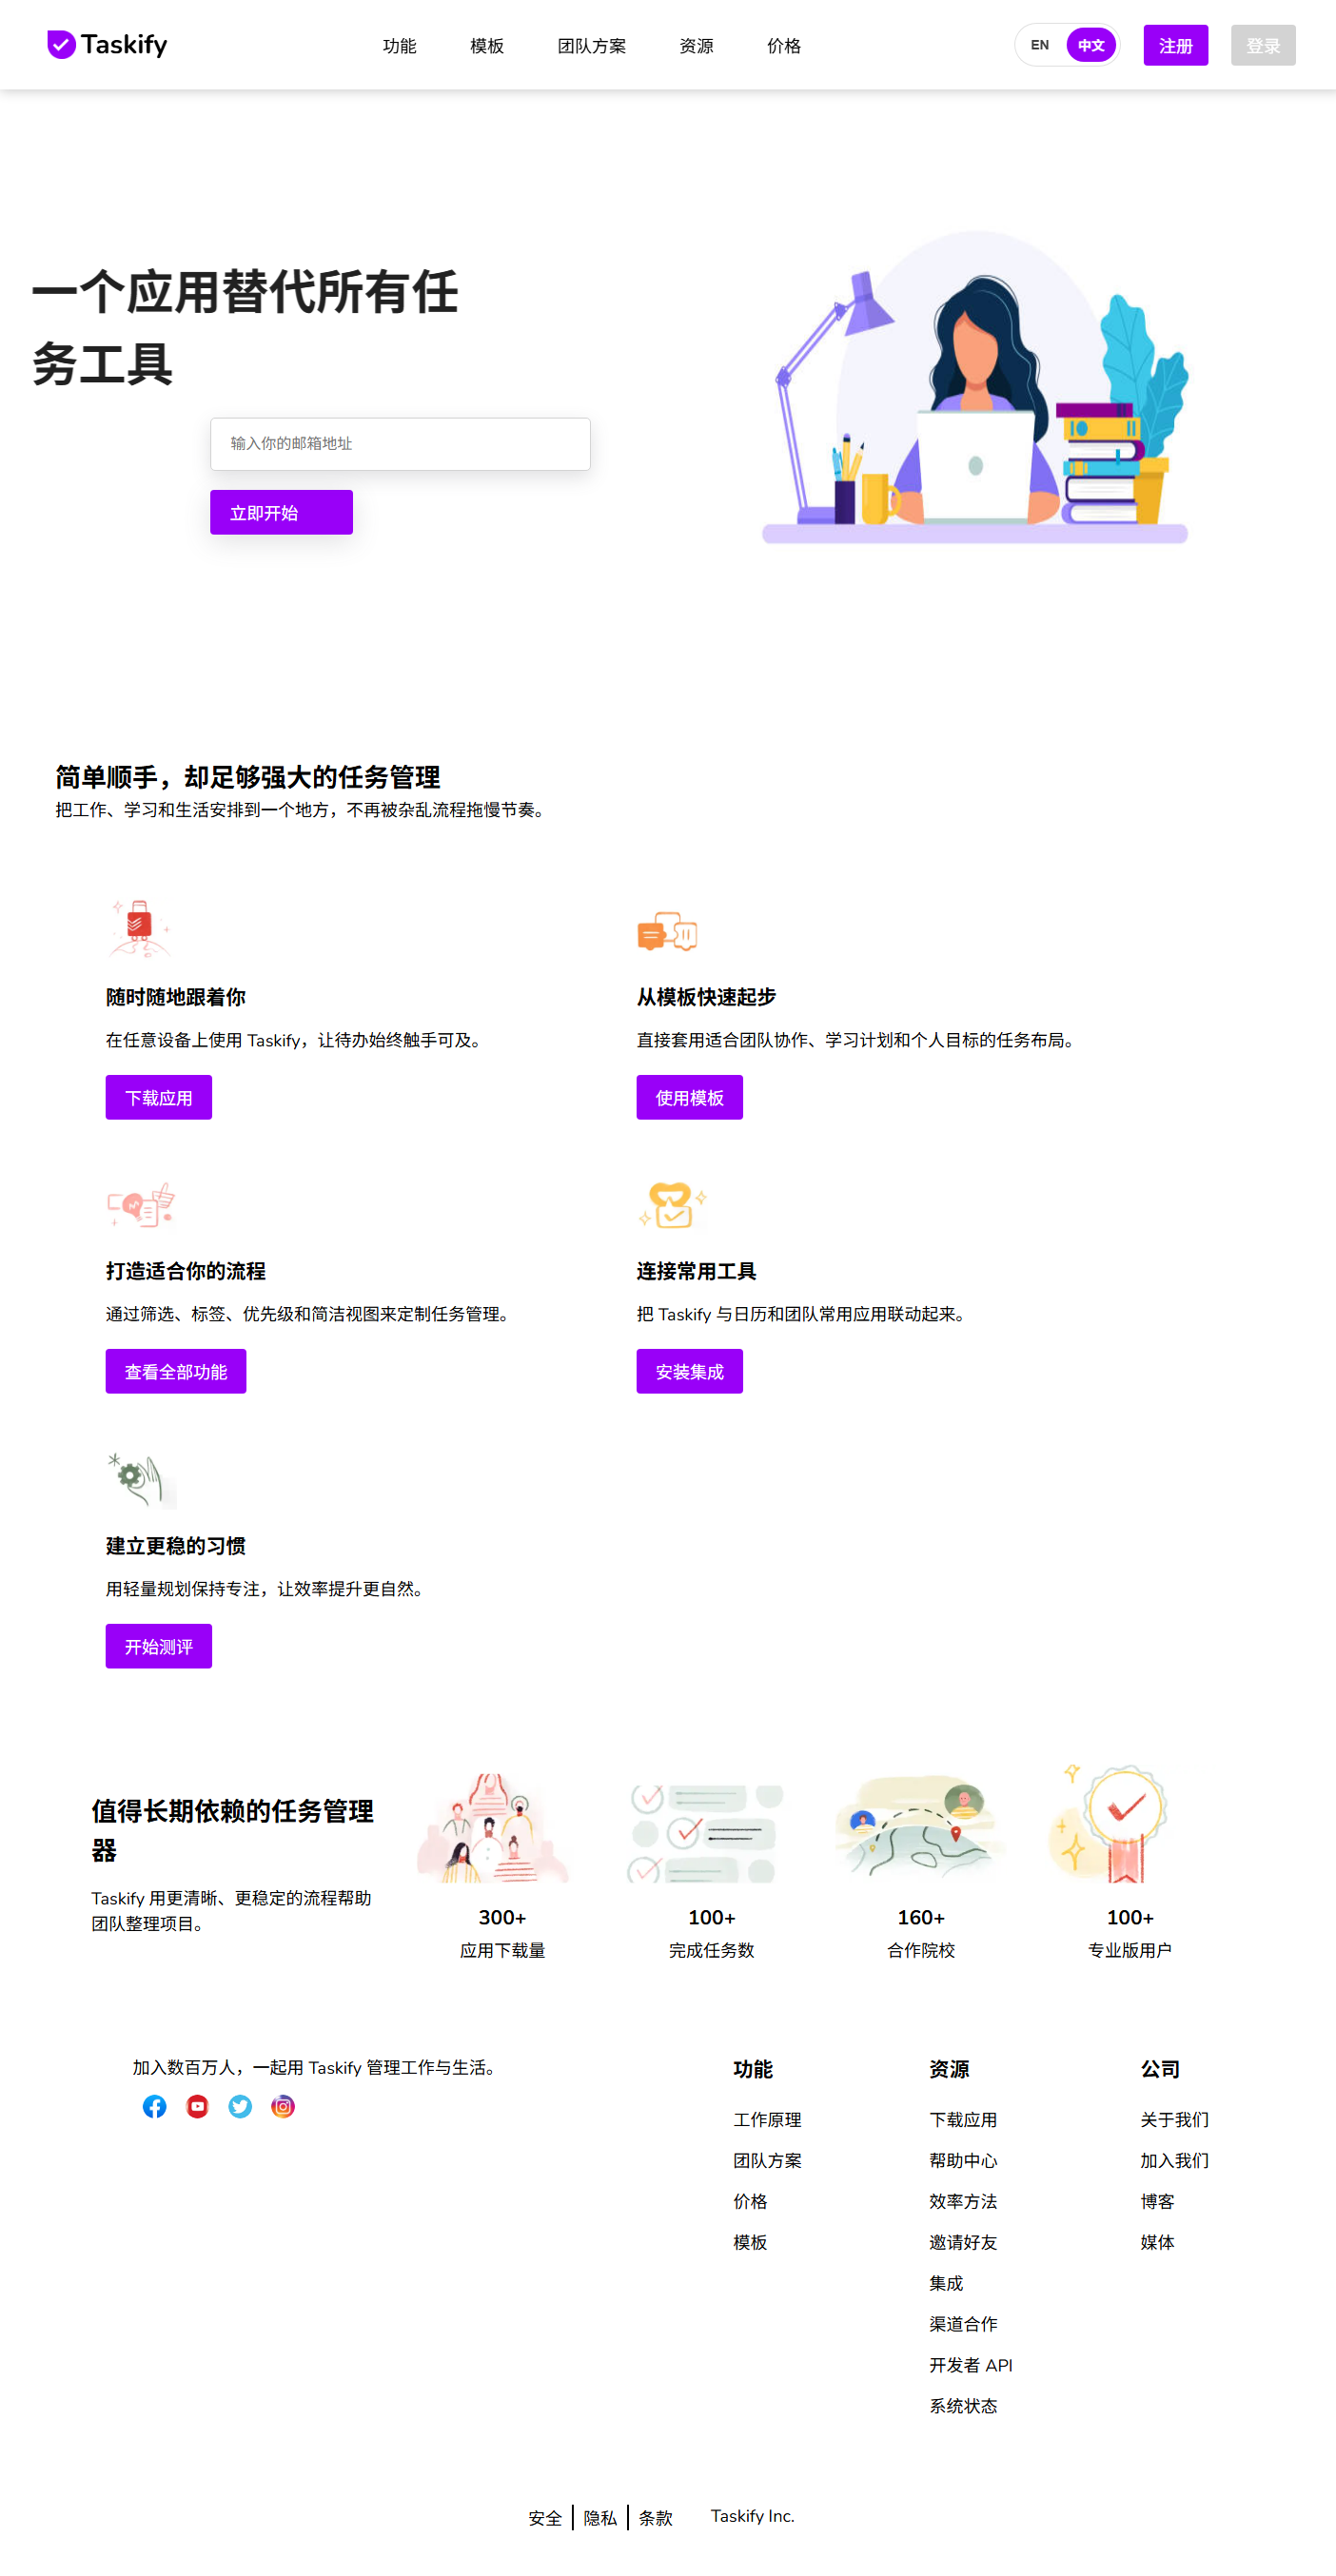
\includegraphics[width=0.92\linewidth]{docs/pr3/evidence/home-zh.png}
  \caption{Internationalization evidence. The language toggle switches the homepage into Chinese, demonstrating a working bilingual interface.}
  \label{fig:language-toggle}
\end{figure}

\begin{figure}[H]
  \centering
  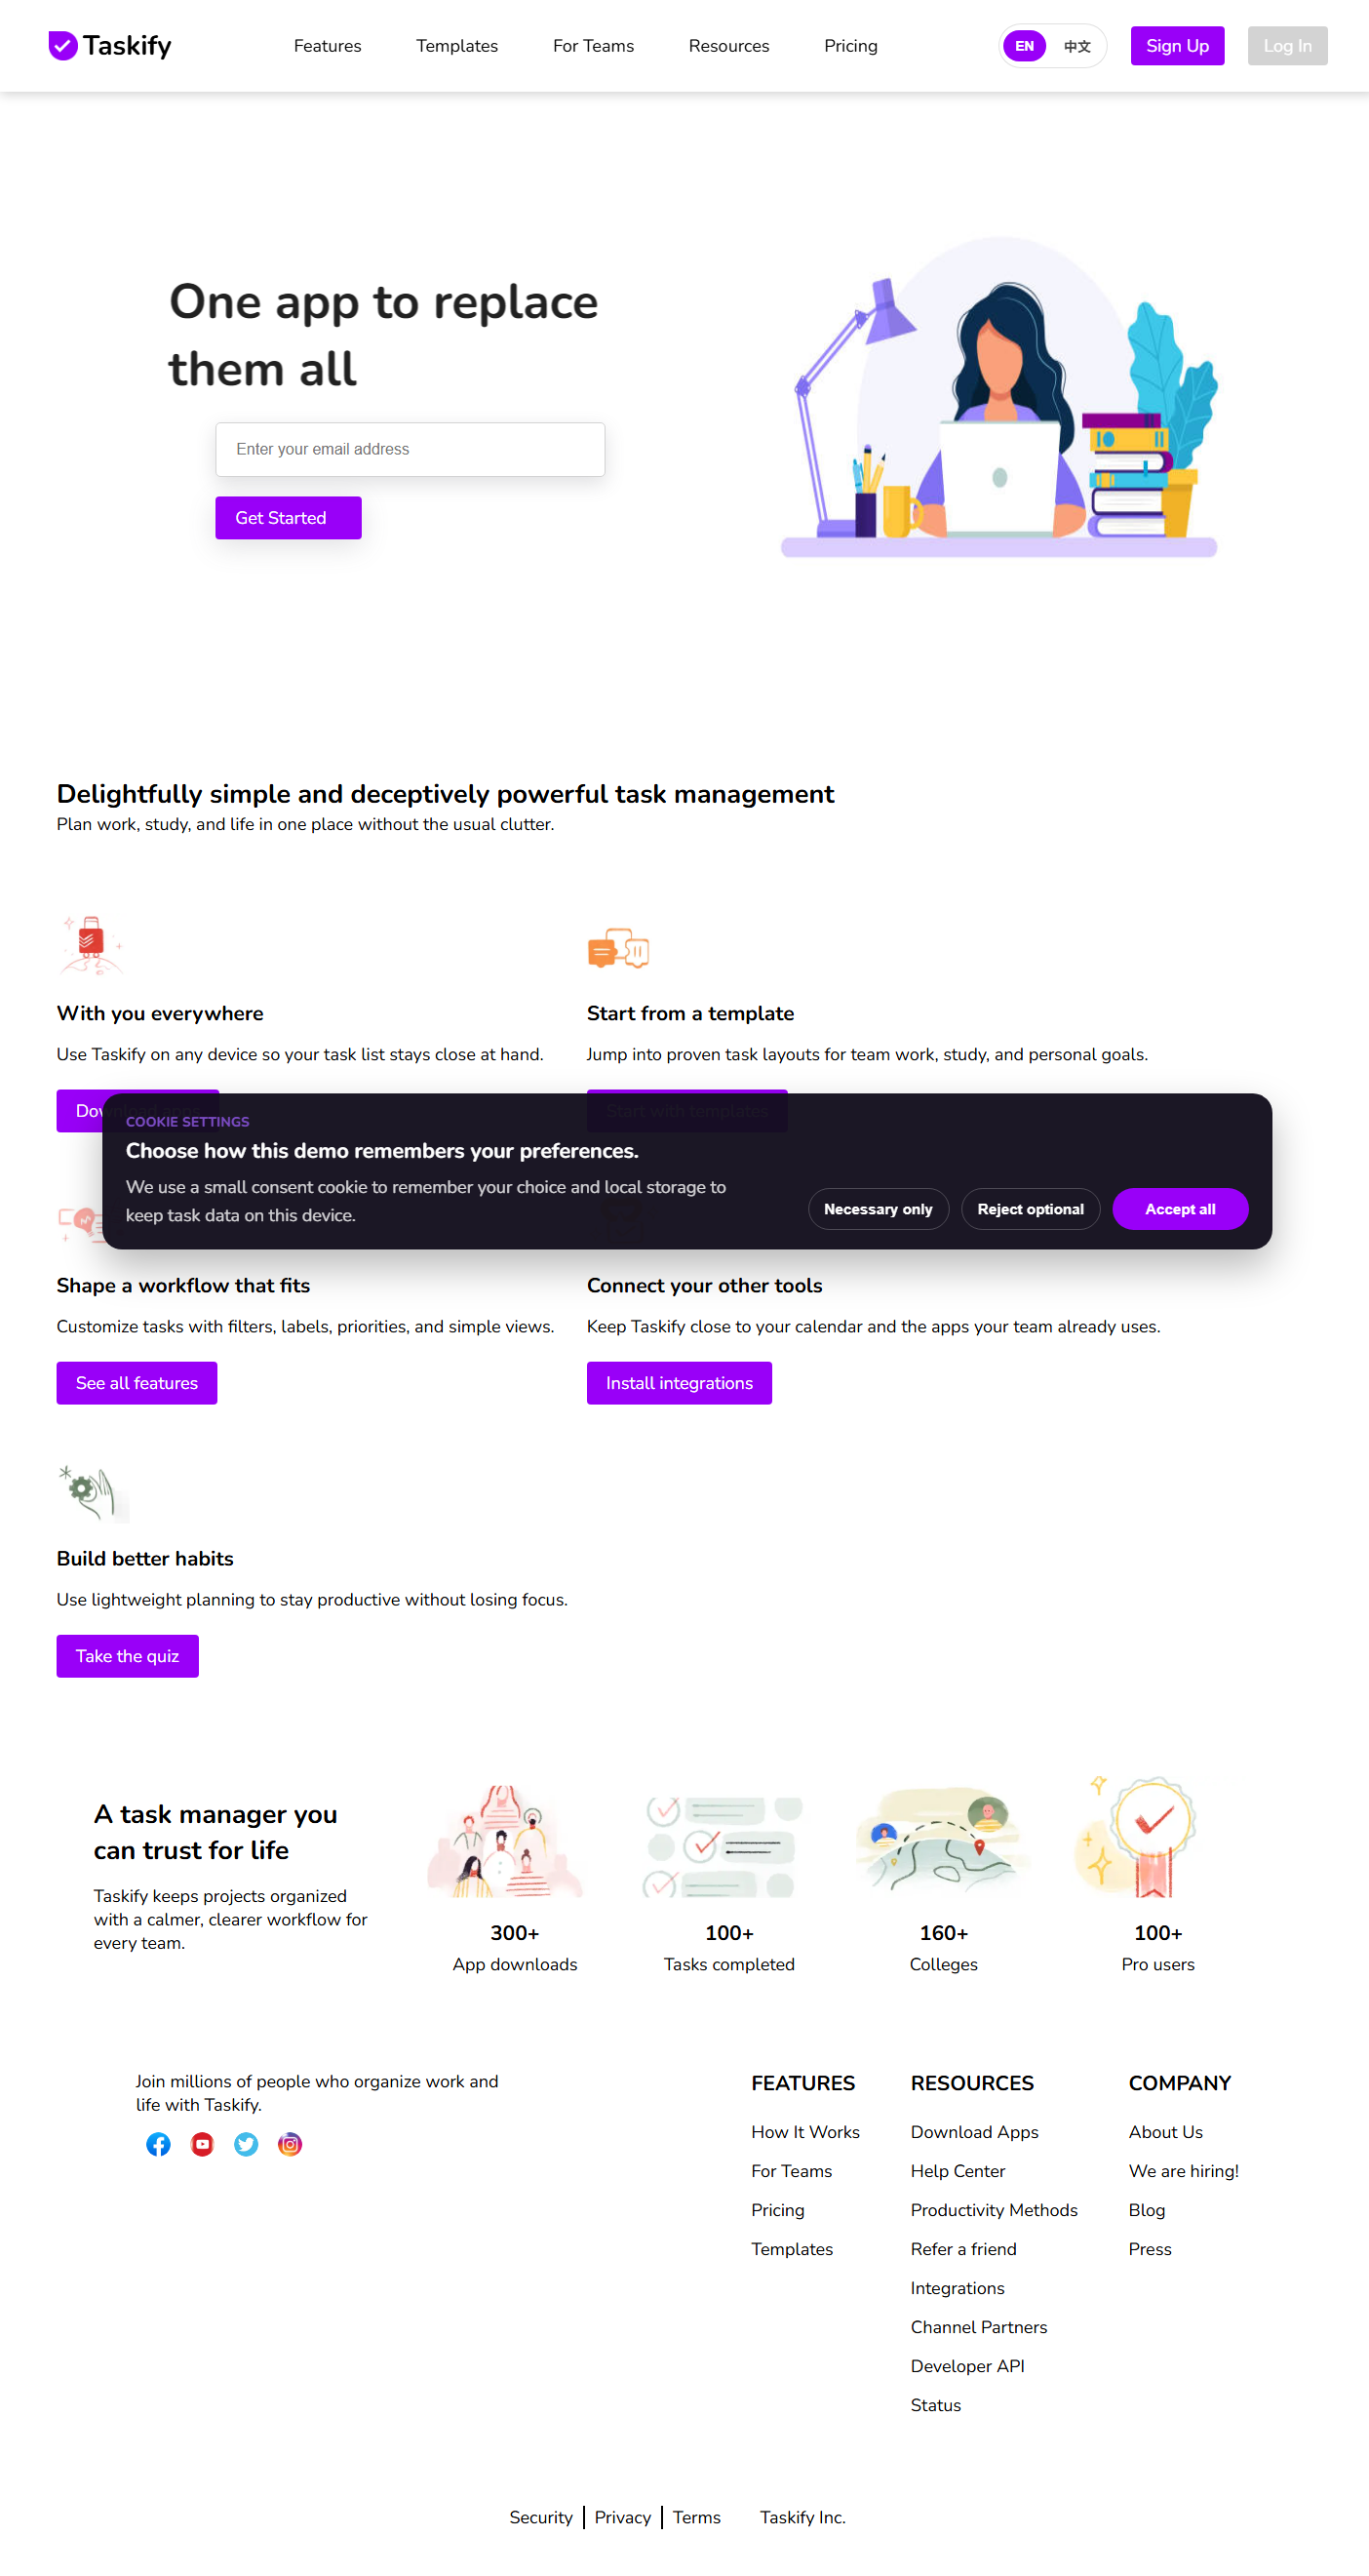
\includegraphics[width=0.92\linewidth]{docs/baseline/evidence/cookie-banner.png}
  \caption{Cookie-banner evidence for legal compliance. The delivered site shows a functional consent banner to visitors.}
  \label{fig:cookie-banner}
\end{figure}

\begin{figure}[H]
  \centering
  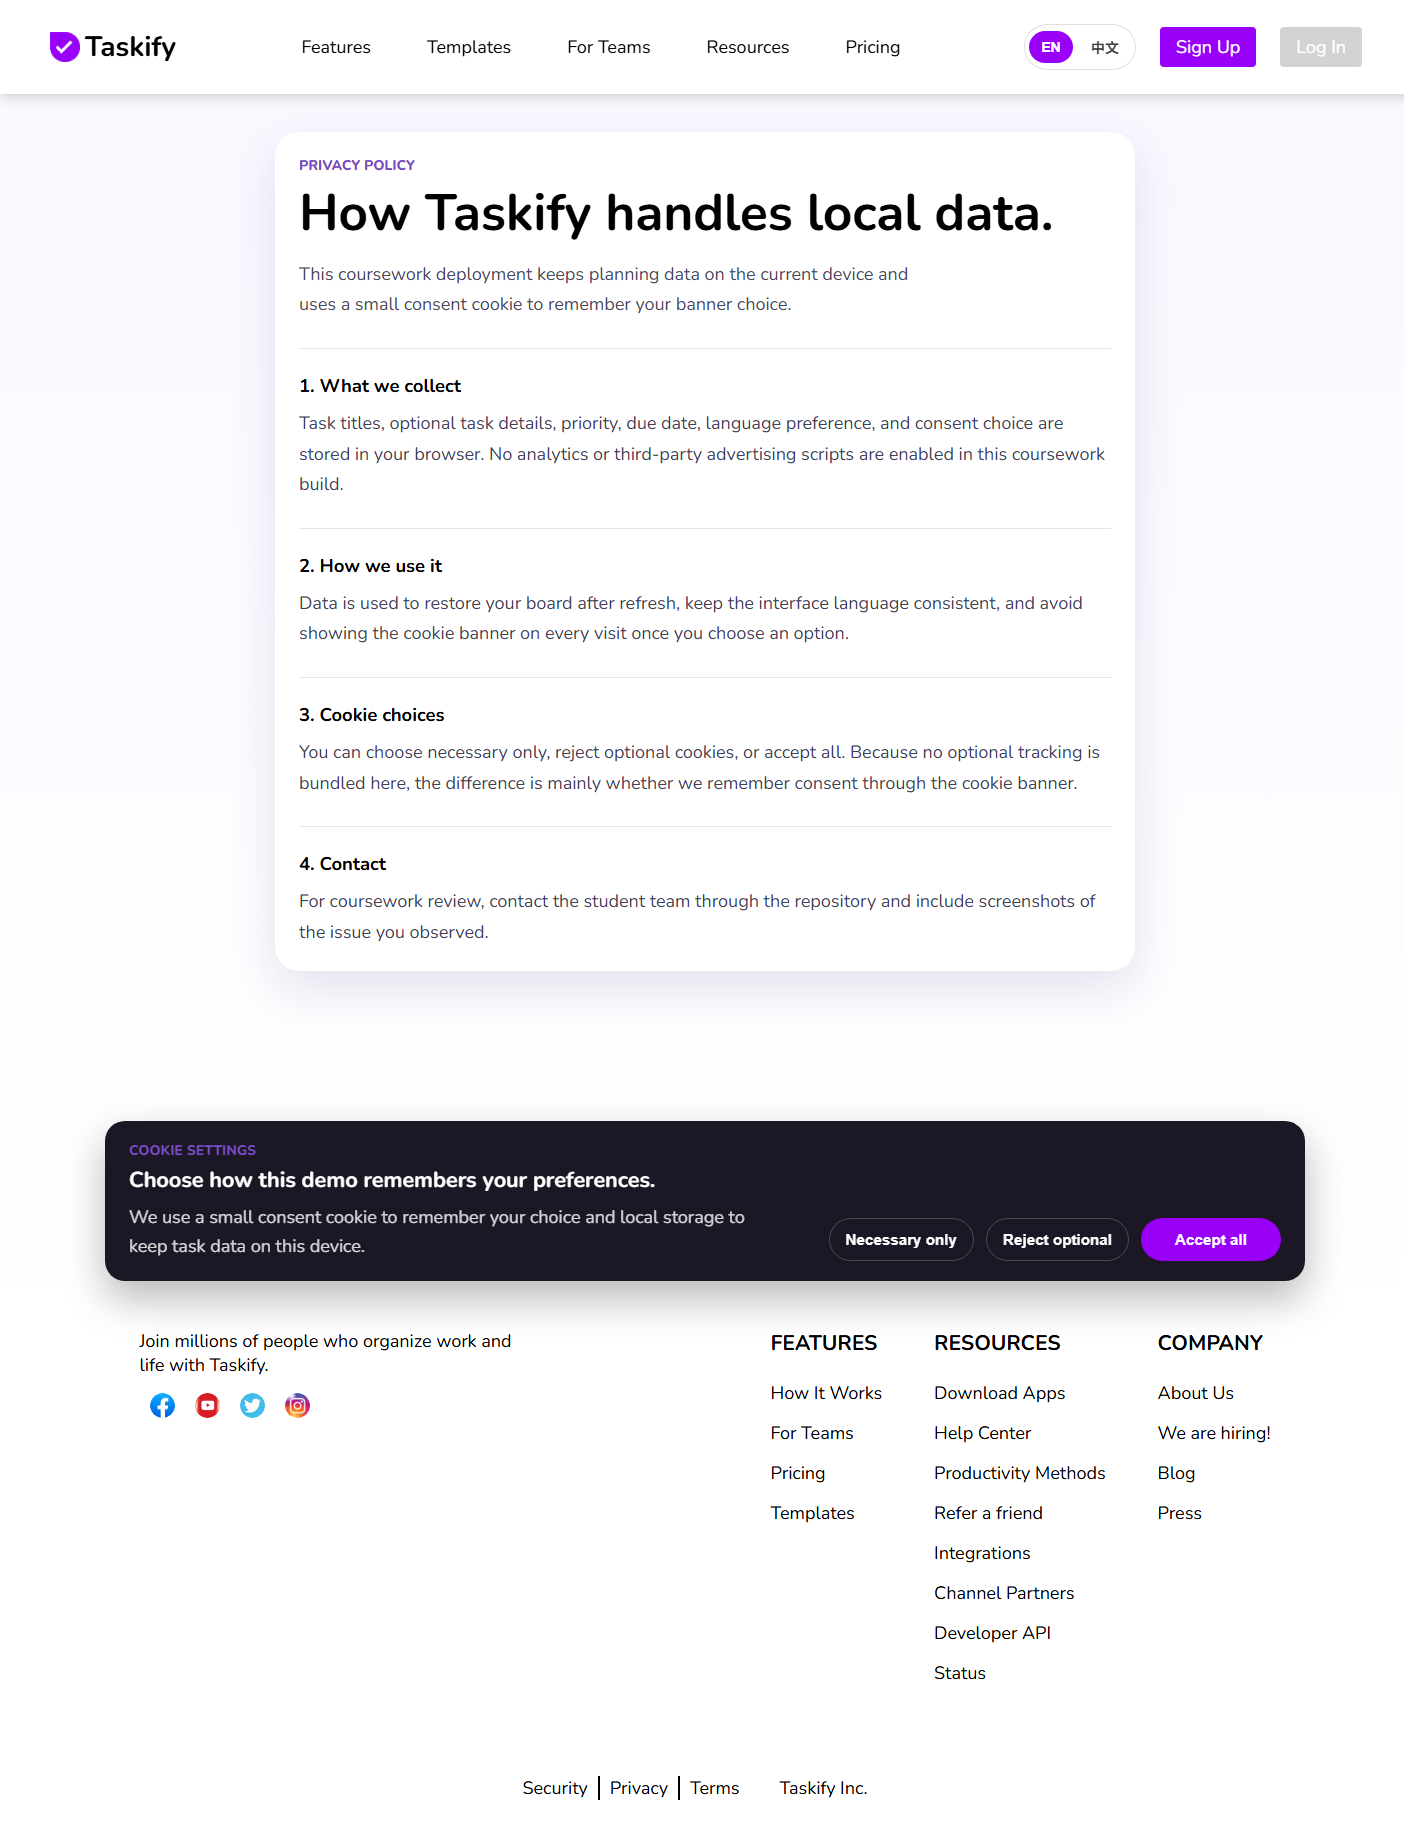
\includegraphics[width=0.92\linewidth]{docs/baseline/evidence/privacy-page.png}
  \caption{Privacy-page evidence for the legal-compliance baseline. The delivered application includes a dedicated privacy-policy page alongside the cookie banner.}
  \label{fig:privacy-page}
\end{figure}

\section{Individual Contribution Forms}

\begin{figure}[p]
  \centering
  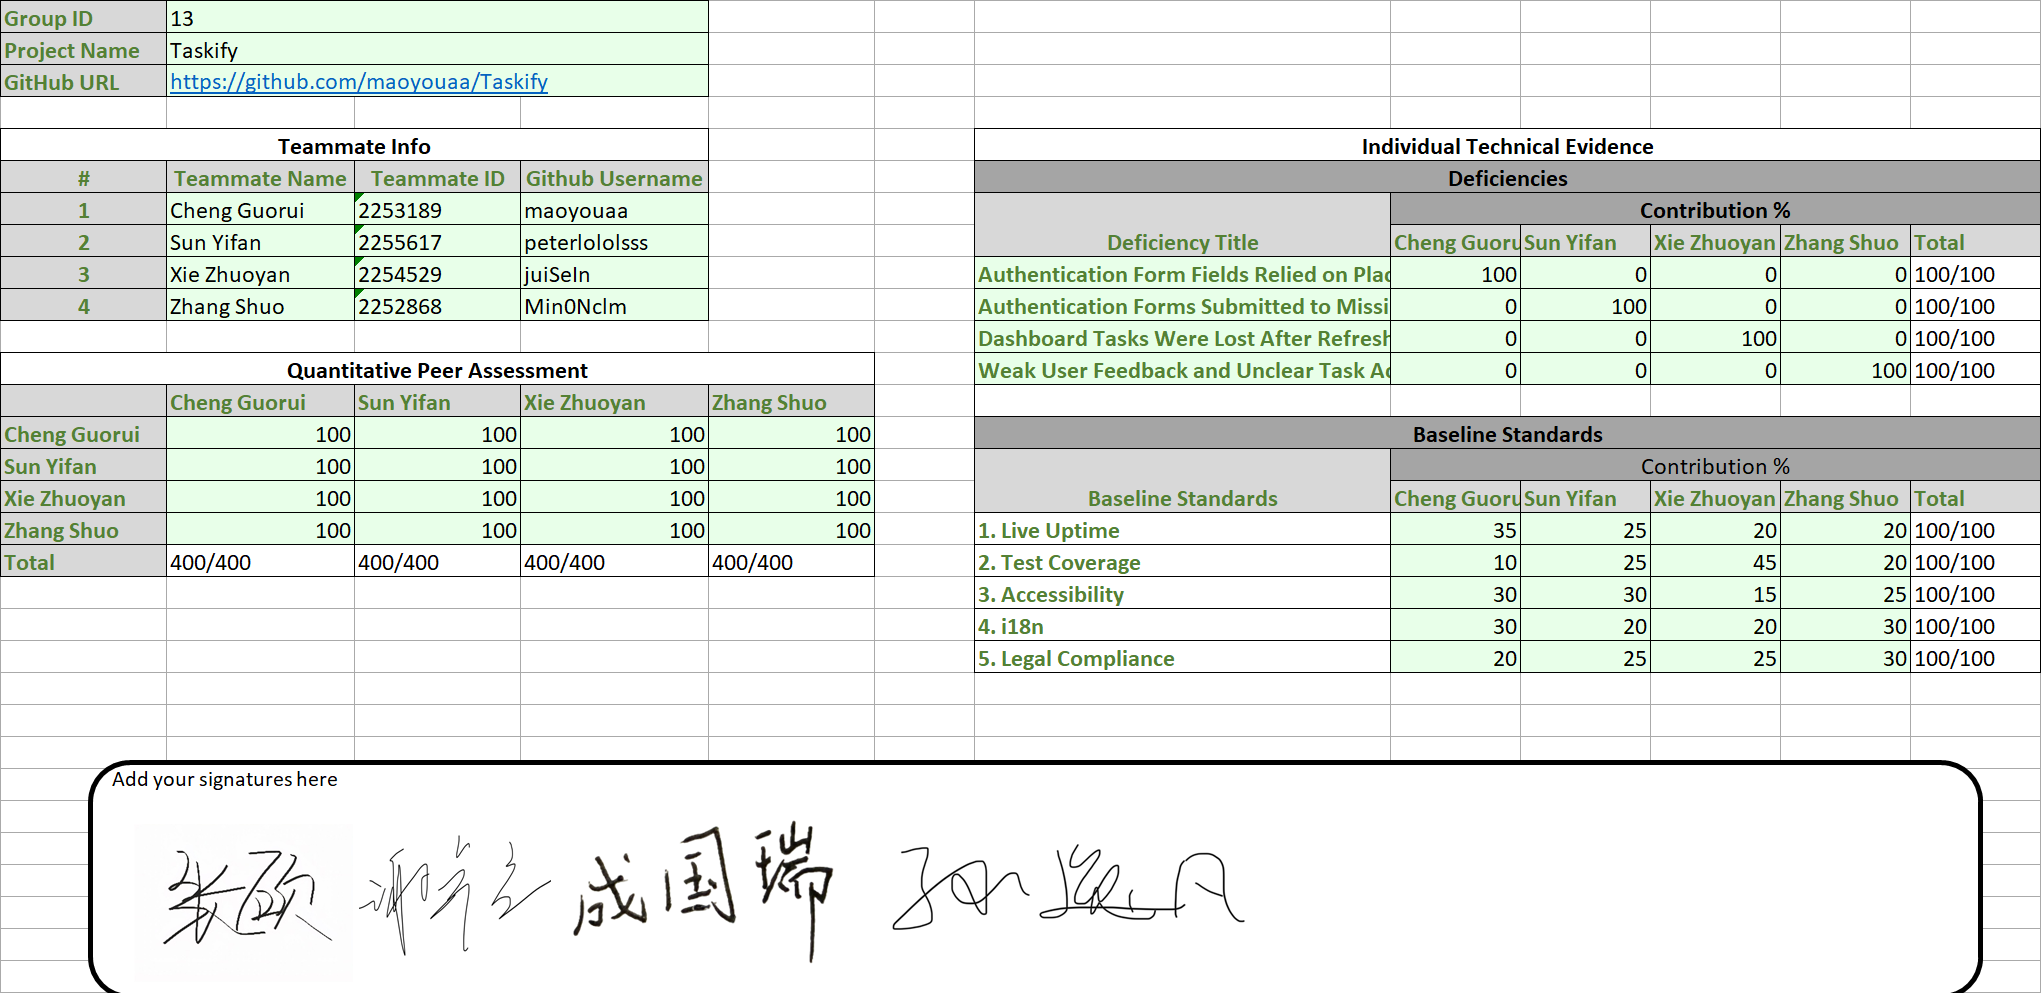
\includegraphics[width=\linewidth,height=0.93\textheight,keepaspectratio]{figures/individual-contribution-form-signed.png}
\end{figure}

\clearpage

\section{References}
\renewcommand{\refname}{}
\vspace{-2em}
\begin{thebibliography}{12}
\bibitem{w3c-labels} W3C Web Accessibility Initiative, ``Labeling Controls,'' Forms Tutorial. [Online]. Available: \url{https://www.w3.org/WAI/tutorials/forms/labels/}. Accessed: May 8, 2026.
\bibitem{webaim-forms} WebAIM, ``Creating Accessible Forms - Advanced Form Labeling.'' [Online]. Available: \url{https://webaim.org/techniques/forms/advanced}. Accessed: May 8, 2026.
\bibitem{w3c-sc332} W3C Web Accessibility Initiative, ``Understanding Success Criterion 3.3.2: Labels or Instructions.'' [Online]. Available: \url{https://www.w3.org/WAI/WCAG22/Understanding/labels-or-instructions.html}. Accessed: May 8, 2026.
\bibitem{express-routing} Express, ``Routing.'' [Online]. Available: \url{https://expressjs.com/en/guide/routing.html}. Accessed: May 8, 2026.
\bibitem{owasp-input-validation} OWASP Cheat Sheet Series, ``Input Validation Cheat Sheet.'' [Online]. Available: \url{https://cheatsheetseries.owasp.org/cheatsheets/Input_Validation_Cheat_Sheet.html}. Accessed: May 8, 2026.
\bibitem{owasp-authentication} OWASP Cheat Sheet Series, ``Authentication Cheat Sheet.'' [Online]. Available: \url{https://cheatsheetseries.owasp.org/cheatsheets/Authentication_Cheat_Sheet.html}. Accessed: May 14, 2026.
\bibitem{owasp-session-management} OWASP Cheat Sheet Series, ``Session Management Cheat Sheet.'' [Online]. Available: \url{https://cheatsheetseries.owasp.org/cheatsheets/Session_Management_Cheat_Sheet.html}. Accessed: May 14, 2026.
\bibitem{mdn-303} MDN Web Docs, ``303 See Other.'' [Online]. Available: \url{https://developer.mozilla.org/en-US/docs/Web/HTTP/Reference/Status/303}. Accessed: May 8, 2026.
\bibitem{mdn-localstorage} MDN Web Docs, ``Window: localStorage property.'' [Online]. Available: \url{https://developer.mozilla.org/en-US/docs/Web/API/Window/localStorage}. Accessed: May 9, 2026.
\bibitem{webdev-storage} web.dev, ``Storage for the web.'' [Online]. Available: \url{https://web.dev/storage-for-the-web/}. Accessed: May 9, 2026.
\bibitem{barrington-usable-products} S. Barrington, ``Usability in the Lab: Techniques for Creating Usable Products,'' \textit{Journal of Laboratory Automation}, vol. 12, no. 1, 2007. [Online]. Available: \url{https://doi.org/10.1016/j.jala.2006.08.004}. Accessed: May 8, 2026.
\bibitem{nngroup-heuristics} Nielsen Norman Group, ``10 Usability Heuristics for User Interface Design.'' [Online]. Available: \url{https://www.nngroup.com/articles/ten-usability-heuristics/}. Accessed: May 17, 2026.
\end{thebibliography}

\end{document}

